\subsection{The Approximate Nearest Neigbour Problem}\label{subsec:approximate_nearest_neighbour_problem}

For all definitions of the NN and its variants, a set of $n$ points $P = \{p_1, \dots, p_n \}$ in a metric space $(X, d)$ where $P \subset X$ is considered.\footnote{It is assumed that $d$ is a proper \textit{metric}, which means that it is \textit{symmetric}: $d(p,q)=d(q,p)$ , \textit{reflexive}: $d(p,q) \leq 0$, $d(p,q)=0 \iff p=q$ and satisfies the \textit{triangle inequality}: $d(p,q) \leq d(p,s) + d(s,q)$.} Then, the general NN is stated as follows.

\begin{definition}[Nearest Neigbour Problem]\label{def:nn}
     Construct a data structure so as to efficiently answer the following query: Given any query point $q$, find some point $p \in P$ such that
    \begin{equation}
        \mathop{\text{min}}_{q \in X} \; d(p, q).
    \end{equation}
\end{definition}

A specific example of Definition \ref{def:nn} could include high-dimensional data in $P \in \mathbb{R}^k$ with $k \gg 1$ and define $d$ as the euclidean distance. In this case, an exhaustive search would require a query time of $O(kn)$. Unfortunately, all exact algorithms that provide a better time complexity than an exhaustive search require $O(2^k)$ space \cite{rubinstein2018hardness}. This tradeoff between time and space complexity is usually referred to as ``curse of dimensionality'' and can only be resolved by accepting approximate solutions. The $c$-approximate nearest neighbour problem ($c$-ANN) is defined as follows.

\begin{definition}[$c$-Approximate Nearest Neighbour Problem]
    For any given query point $q \in X$ and some approximation factor $c > 1$, find some point $p \in P$ such that
    \begin{equation}
        d(q,p) < c \cdot \mathop{\text{min}}_{s \in P} \; d(s, q).
    \end{equation}
\end{definition}

Thus, the distance from the query point $q$ to the approximate nearest neighbour $p$ is at most $c$ times the distance to the true nearest neighbour $s$. Strictly speaking, LSH does not solve the $c$-ANN directly. Instead, Indyk and Motwani relaxed the problem by introducing the $cR$-approximate nearest neighbour problem ($cR$-ANN) as follows.

\begin{definition}[$cR$-Approximate Nearest Neighbour Problem]
    For any given query point $q \in X$, some approximation factor $c > 1$ and some target distance $R > 0$, if there exists a point $p \in P$ where $d(p,q) \leq R$, then return a point $p' \in P$ where
    \begin{equation}
        d(p',q) \leq cR.
    \end{equation}
\end{definition}

Figure \ref{fig:nearest_neighbour} illustrates  the $cR$-ANN. The target distance $R$ represents the distance of the query object from its nearest neighbour. If there is such a point, the algorithm returns points within $cR$ distance from the query object. Otherwise it returns nothing. It is shown that LSH can solve the $c$-ANN by solving the $cR$-ANN for different settings of $R$ \cite{indyk_approximate_1998}.

\begin{figure}[t!]
    \centering
    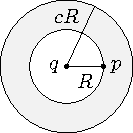
\includegraphics[width=0.3\linewidth]{tikz/nearest_neighbour.pdf}
    \caption{In the $cR$-approximate nearest neighbour problem some point within $cR$ is accepted, if there exists a point $p$ where $d(p,q) \leq R$.}
    \label{fig:nearest_neighbour}
\end{figure}